% +------------------------------------------------------------------------+
% | Reference manual page: Subdivision_surfaces_3.tex
% +------------------------------------------------------------------------+
% | 03/01/2005   Le-Jeng Andy Shiue
% | Package: Subdivision_surface_3
% | 
\RCSdef{\RCSSubdivisionRev}{$Revision$}
\RCSdefDate{\RCSSubdivisionDate}{$Date$}
% +------------------------------------------------------------------------+

\ccRefPageBegin

%%RefPage: end of header, begin of main body
% +------------------------------------------------------------------------+


\begin{ccRefClass}{Subdivision_surfaces_3<Poly>}

\ccDefinition

Subdivision surfaces of an input polyhedral mesh
are generated by recursive topology refinement and geometry
smoothing. \ccClassTemplateName\ consists of a set of static 
template functions. These functions implements refinement schemes 
practically used by subdivision algorithms. These functions,
called refinement hosts, work only on the connectivity of the
control mesh. The assignment of
the \emph{smoothed} geometry is dedicated to the user-customizable
policy class. Each refinement host is parameterized with a 
policy class. This class consists of a set of functions realizing
the geometry masks. 
%specifically developed to fit the refinement pattern.
%consisting of a set of geometry stencils, 
The host refines the control mesh, maintains the stencils, and assigns the 
geometry of the refined mesh by calling the policy functions.

Primal-Quadrilateral-Quadrisection (PQQ), Primal-Triangle-Quadrisection 
(PTQ), Dual-Quadrilateral-Quadrisection (DQQ), and $\sqrt{3}$ triangulation
are supported in \ccClassTemplateName . Each of these refinements are used in 
Catmull-Clark, Loop, Doo-Sabin and $\sqrt{3}$ subdivision, respectively. 

%% \begin{ccTexOnly}
%%     \vspace{-7mm}
%%     \begin{center}
%%       \parbox{0.4\textwidth}{%
%%         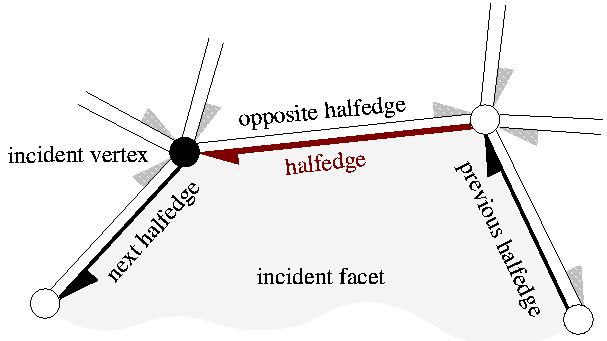
\includegraphics[width=0.4\textwidth]{Polyhedron_ref/fig/halfedge}%
%%       }
%%     \end{center}
%%     \vspace{-5mm}
%% \end{ccTexOnly}

%% \begin{ccHtmlOnly}
%%     <CENTER>
%%     <A HREF="fig/halfedge.gif">
%%         <img src="fig/halfedge_small.gif" alt="Halfedge Diagram"></A><P>
%%     </CENTER>
%% \end{ccHtmlOnly}

\ccInclude{CGAL/Subdivision_surfaces_3.h}

\ccParameters

The full template declaration of \ccClassTemplateName\ states one
template parameters:

\begin{tabbing}
\ccc{template <} \=\ccc{class Polyhedron_3>} \ccc{class Subdivision_surfaces_3;}
\end{tabbing}
   
The parameter \ccc{Polyhedron_3} requires a model of 
the \ccc{Polyhedron_3} concept as argument. The storage structure
of \ccc{Polyhedron_3} is required to be a FIFO structure (e.g.~vector 
or list), and the order of the primitive iteration is assumed in the order
of the primitive insertion. This storage condition avoids the requirement 
of explicit tags to maintain the stencils since refined nodes are 
generated in a specific order that is used to enumerate the stencils. 
To work on the geometry smoothing, 
\ccc{Point_3} is required to be defined in the \ccc{Polyhedron_3} as the 
geometry attribute of each vertex.

%% \ccTypes

%% \ccNestedType{Traits}{traits class selected for \ccc{PolyhedronTraits_3}.}
%% \ccGlue
%% \ccNestedType{Items}{items class selected for \ccc{PolyhedronItems_3}.}
%% \ccGlue



%% % +-----------------------------------+
%% \begin{ccAdvanced}
%% \ccHeading{Types for Tagging Optional Features}

%% \ccNestedType{Supports_facet_plane}{\ccc{Facet::plane()}.}
%% \ccGlue
%% \ccNestedType{Supports_removal}{supports removal of individual elements.}

%% \end{ccAdvanced}

\ccCreation
\ccCreationVariable{S}

\ccClassTemplateName\ serves as a template namespace, hence no constructor
is defined. 

%and provides a 
%set of static functions of refinements. 

%No object of \ccClassTemplateName\ is reuqired to be 
%instantiated before calling subdivision or generic refinement functions.

% +-----------------------------------+
\ccHeading{Refinement hosts}

All refinement hosts are static template functions in the format of
\ccc{template <template <typename> class Stencil> void RefHost(...);}.
Primal-Quadrilateral-Quadrisection (PQQ), Primal-Triangle-Quadrisection 
(PTQ), Dual-Quadrilateral-Quadrisection (DQQ), and $\sqrt{3}$ triangulation
are supported.

%\ccThree{void}{S::PQQ(Poly& p, Stencil<Poly> rule, int s);}{}
%\ccThreeToTwo
\ccTwo{template <template <typename> class Stencil> void PQQ(Poly& p, Stencil<Poly> rule, int s);}{}

\ccThree{template <template <typename> class Stencil> void}{sub}{}
\ccThreeToTwo


\ccFunction{
template <template <typename> class Stencil>
void PQQ(Poly& p, Stencil<Poly> rule, int d);
}{
refine the mesh \ccc{p} with the PQQ refinement
\ccc{d} times, and assign the geometry of the refined \ccc{p} 
with the geometry masks \ccc{rule}.
}
%% \begin{ccTexOnly}
%%     \begin{center}
%%       \parbox{0.636\textwidth}{%
%%           \includegraphics[width=0.636\textwidth]%
%%               {Polyhedron_ref/fig/euler_loop}%
%%       }
%%     \end{center}
%% \end{ccTexOnly}
%% \begin{ccHtmlOnly}
%%     <CENTER>
%%     <img src="fig/euler_loop.gif" alt="Euler Operator: Loop"><P>
%%     </CENTER>
%% \end{ccHtmlOnly}

\ccFunction{
template <template <typename> class Stencil>
void PTQ(Poly& p, Stencil<Poly> rule, int d);
}{
refine the mesh \ccc{p} with the PTQ refinement 
\ccc{d} times, and assign the geometry of the refined \ccc{p} with 
the geometry masks \ccc{rule}.
}

\ccFunction{
template <template <typename> class Stencil>
void DQQ(Poly& p, Stencil<Poly> rule, int d);
}{
refine the mesh \ccc{p} with the DQQ refinement 
\ccc{d} times, and assign the geometry of the refined \ccc{p} with 
the geometry masks \ccc{rule}.
}

\ccFunction{
template <template <typename> class Stencil>
void Sqrt3(Poly& p, Stencil<Poly> rule, int d);
}{
refine the mesh \ccc{p} with the $\sqrt{3}$ triangulation 
\ccc{d} times, and assign the geometry of the refined \ccc{p} with 
the geometry masks \ccc{rule}.
}


% +-----------------------------------+
\ccHeading{Subdivision Surfaces}

Certain subdivision surfaces are widely used in geometry modeling
and computer graphics. A set of subdivision functions are directly 
provided for these schemes. 
%These subdivision functions are 
%pre-parameterized with their subdivision policies.

%\ccTwo{void CatmullClark_subdivision(Poly& p, int d);}{}
\ccThree{void}{sub}{}
\ccThreeToTwo

\ccFunction{
void CatmullClark_subdivision(Poly& p, int d);
}{
apply Catmull-Clark subdivision \ccc{d} times on the mesh \ccc{p}.
}

\ccFunction{
void Loop_subdivision(Poly& p, int d);
}{
apply Loop subdivision \ccc{d} times on the mesh \ccc{p}. 
The mesh \ccc{p} can only consist of triangle facets.
}

\ccFunction{
void DooSabin_subdivision(Poly& p, int d);
}{
apply Doo-Sabin subdivision \ccc{d} times on the mesh \ccc{p}.
}

\ccFunction{
void Sqrt3_subdivision(Poly& p, int d);
}{
apply $\sqrt{3}$ subdivision \ccc{d} times on the mesh \ccc{p}.
The mesh \ccc{p} can only consist of triangle facets.
}

\ccExample

This example program applies the Catmull-Clark subdivision on a
read-in polyhedral mesh.

\ccIncludeExampleCode{Subdivision_surfaces_3/CatmullClark_subdivision.C}

\ccSeeAlso

\ccRefIdfierPage{CGAL::PQQ_stencil_3<Poly>}\\
\ccRefIdfierPage{CGAL::DQQ_stencil_3<Poly>}\\
\ccRefIdfierPage{CGAL::Linear_stencil_3<Poly>}\\
\ccRefIdfierPage{CGAL::CatmullClark_stencil_3<Poly>}\\
\ccRefIdfierPage{CGAL::Loop_stencil_3<Poly>}\\
\ccRefIdfierPage{CGAL::Sqrt3_stencil_3<Poly>}\\

\end{ccRefClass}

% +------------------------------------------------------------------------+
%%RefPage: end of main body, begin of footer
\ccRefPageEnd
% EOF
% +------------------------------------------------------------------------+
